\documentclass[aspectratio=169]{beamer}
\usetheme{default}
\usecolortheme{dove}
\usepackage{amsmath,amssymb}
\usepackage{graphicx}
\usepackage{booktabs}
\usepackage{tikz}
\usetikzlibrary{arrows.meta,positioning,calc}
\usepackage{xcolor}
\usepackage{hyperref}

\graphicspath{{../pyScripts/dec_6_revision/new_notebooks/results/paper_figs/}}

% Color palette
\definecolor{sigblue}{RGB}{31,119,180}
\definecolor{sigred}{RGB}{214,39,40}
\definecolor{siggreen}{RGB}{44,160,44}
\definecolor{sigorange}{RGB}{255,127,14}
\definecolor{sigpurple}{RGB}{148,103,189}
\definecolor{lightgray}{RGB}{240,240,240}

\setbeamertemplate{navigation symbols}{}
\setbeamertemplate{footline}[frame number]
\setbeamercolor{frametitle}{fg=sigblue}
\setbeamerfont{frametitle}{series=\bfseries}

\newcommand{\aladyn}{\texttt{ALADYNOULLI}}

\title{\textbf{\aladyn{}:\\A Bayesian Framework for Genomic Discovery\\ and Clinical Prediction}}
\subtitle{Disease Signatures, Individual Trajectories, and Drug Discovery}
\author{Sarah M.\ Urbut\textsuperscript{1,2,3,4} \and Pradeep Natarajan\textsuperscript{1,2,3,4}}
\institute{
\textsuperscript{1}Mass General Hospital \quad
\textsuperscript{2}Cardiovascular Research Center \quad
\textsuperscript{3}Harvard Medical School\\
\textsuperscript{4}Broad Institute \quad
\textsuperscript{5}Dana-Farber \quad
\textsuperscript{10}Harvard T.H.\ Chan
}
\date{}

\begin{document}

% ============================================================
% TITLE
% ============================================================
\begin{frame}
\titlepage
\end{frame}

% ============================================================
% OUTLINE
% ============================================================
\begin{frame}{Outline}
\begin{enumerate}
    \item \textbf{The problem}: Disease complexity across 348 conditions over a lifetime
    \item \textbf{The model}: \aladyn{} --- signatures, trajectories, genetics
    \item \textbf{Discovery}: Consistent signatures across 3 biobanks (700K+ patients)
    \item \textbf{Heterogeneity}: Different pathways to the same diagnosis
    \item \textbf{Genetics}: 151 GWAS loci, rare variants, heritability
    \item \textbf{Prediction}: Outperforming PCE, PREVENT, GAIL across 28 diseases
    \item \textbf{Applications}: Patient stratification, trial design, drug targets
\end{enumerate}
\end{frame}

% ============================================================
% THE PROBLEM
% ============================================================
\begin{frame}{The Problem: Disease Doesn't Happen in Isolation}
\begin{columns}
\begin{column}{0.55\textwidth}
\textbf{A real patient's journey:}
\begin{itemize}
    \item Rheumatoid arthritis at age 45
    \item Hypertension at 48
    \item Myocardial infarction at 52
\end{itemize}
\vspace{8pt}
\textbf{Traditional approaches:}
\begin{itemize}
    \item Treat each disease in isolation
    \item Miss the underlying metabolic-inflammatory process
    \item Separate risk models for each condition
    \item Cannot share information across related diseases
\end{itemize}
\end{column}
\begin{column}{0.42\textwidth}
\textbf{What we need:}
\begin{itemize}
    \item Model \textbf{all 348 diseases} jointly
    \item Capture \textbf{temporal dynamics} across the lifespan
    \item Integrate \textbf{genetics} directly
    \item Share information across \textbf{related conditions}
    \item Provide \textbf{interpretable} biological structure
    \item \textbf{Predict} future disease risk
\end{itemize}
\end{column}
\end{columns}
\end{frame}

% ============================================================
% THE MODEL
% ============================================================
\begin{frame}{The Model: \aladyn{}}
\textbf{Core equation --- mixture of probabilities:}
\vspace{-4pt}
\[
\pi_{idt} = \kappa \cdot \sum_{k=1}^{K} \underbrace{\theta_{ikt}}_{\substack{\text{individual}\\\text{loading}}} \cdot \underbrace{\text{sigmoid}(\phi_{kdt})}_{\substack{\text{signature-disease}\\\text{association}}}
\]
\vspace{-6pt}
\begin{columns}
\begin{column}{0.48\textwidth}
\textbf{Individual trajectories} ($\lambda \to \theta$):
\vspace{-4pt}
\[
\lambda_{ik} \sim \mathcal{GP}\!\left(r_k + \mathbf{g}_i^\top \Gamma_k,\; \Omega_\lambda\right)
\]
\vspace{-8pt}
\begin{itemize}\setlength\itemsep{0pt}
    \item $\mathbf{g}_i$: 36 PRS + sex + 10 PCs
    \item $\Gamma_k$: genetic effects on signature $k$
    \item $\Omega_\lambda$: temporal smoothness
\end{itemize}
\end{column}
\begin{column}{0.48\textwidth}
\textbf{Disease signatures} ($\phi$):
\vspace{-4pt}
\[
\phi_{kd} \sim \mathcal{GP}\!\left(\mu_d + \psi_{kd},\; \Omega_\phi\right)
\]
\vspace{-8pt}
\begin{itemize}\setlength\itemsep{0pt}
    \item $\mu_d$: population baseline prevalence
    \item $\psi_{kd}$: signature-disease strength
    \item $\Omega_\phi$: temporal smoothness
\end{itemize}
\end{column}
\end{columns}
\vspace{4pt}
\centering\small\textcolor{sigblue}{\textbf{Key:}} Diseases conditionally independent given signatures --- correlations mediated through shared biology.
\end{frame}

% ============================================================
% KEY DIFFERENCES
% ============================================================
\begin{frame}{\aladyn{} vs.\ Traditional Approaches}

\begin{center}
\renewcommand{\arraystretch}{1.3}
\begin{tabular}{lcc}
\toprule
\textbf{Feature} & \textbf{Traditional / Topic Models} & \textbf{\aladyn{}} \\
\midrule
Diseases modeled & 1 at a time & \textbf{348 jointly} \\
Temporal dynamics & Static snapshot & \textbf{Age-varying GP} \\
Genetic integration & Post-hoc & \textbf{In the model} \\
Prediction type & Retrospective & \textbf{Prospective} \\
Rare diseases & Insufficient data & \textbf{Borrows strength} \\
Patient description & Risk score (1 number) & \textbf{Signature profile} \\
Bias correction & None & \textbf{IPW via likelihood} \\
Data required & Labs, biomarkers & \textbf{ICD codes only} \\
\bottomrule
\end{tabular}
\end{center}

\end{frame}

% ============================================================
% FIGURE 1 PLACEHOLDER
% ============================================================
\begin{frame}{Model Overview}
\begin{center}
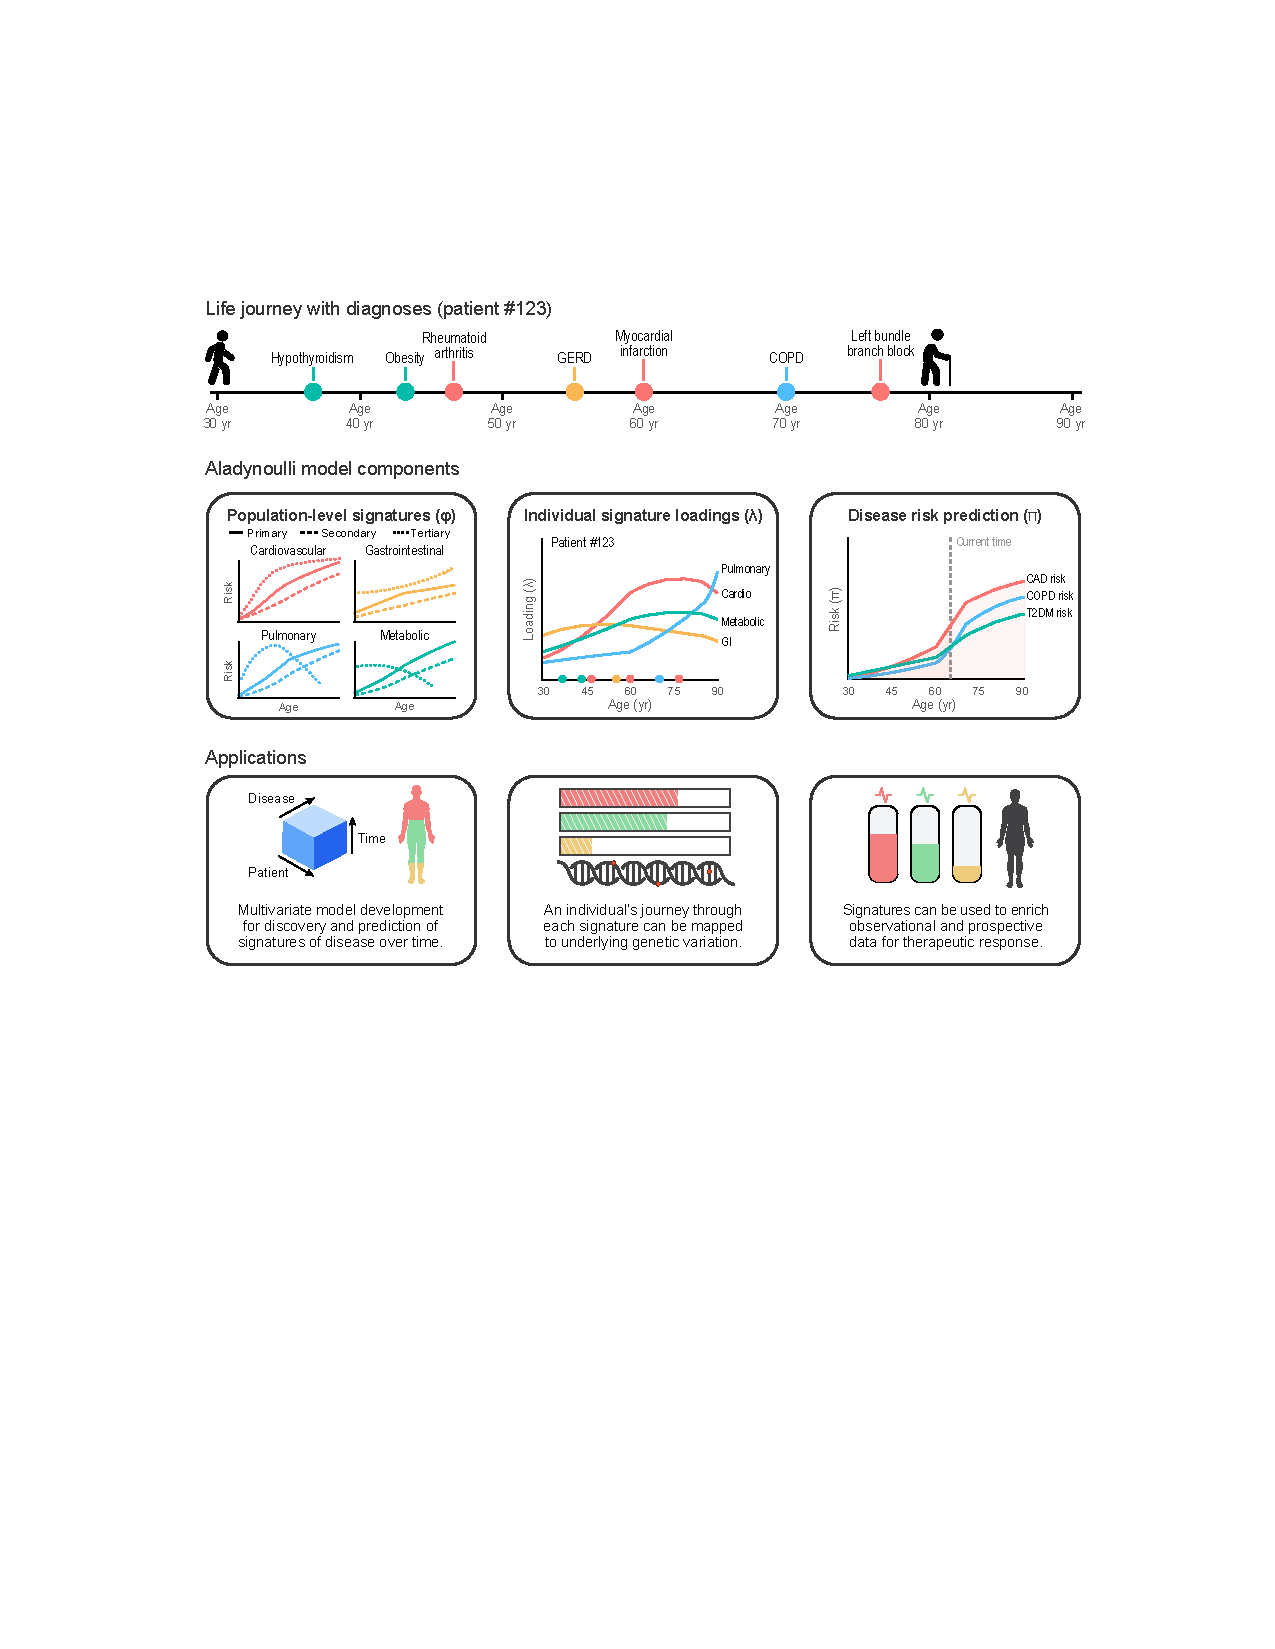
\includegraphics[width=0.85\textwidth,height=0.78\textheight,keepaspectratio]{Fig1.pdf}
\end{center}
\vspace{-6pt}
\small \textit{Top:} Patient timeline. \textit{Middle:} Signatures ($\phi$), loadings ($\theta$), risk ($\pi$). \textit{Bottom:} Applications.
\end{frame}

% ============================================================
% THREE COHORTS
% ============================================================
\begin{frame}{Three Independent Biobanks}

\begin{center}
\renewcommand{\arraystretch}{1.3}
\begin{tabular}{lccc}
\toprule
& \textbf{UK Biobank} & \textbf{Mass General Brigham} & \textbf{All of Us} \\
\midrule
N & 427,239 & 48,069 & 208,263 \\
Follow-up & Up to 52 years & $\sim$30 years & $\sim$6 years \\
EHR from & $\sim$1980 & $\sim$1990 & $\sim$2018 \\
Country & UK & USA (Boston) & USA (national) \\
Diseases & 348 & 346 & 348 \\
Genetics & Array + imputed & Array & WGS + array \\
\bottomrule
\end{tabular}
\end{center}

\vspace{8pt}
\begin{center}
\textcolor{sigblue}{\textbf{Despite different populations, healthcare systems, and data collection ---\\ signatures are remarkably consistent.}}
\end{center}
\end{frame}

% ============================================================
% FIGURE 2: SIGNATURES
% ============================================================
\begin{frame}{Disease Signatures: Temporal Patterns}
\begin{columns}
\begin{column}{0.48\textwidth}
\centering
\includegraphics[width=\textwidth]{fig2/fig2_signature_5.pdf}\\
\small Ischemic Cardiovascular (Sig 5)
\end{column}
\begin{column}{0.48\textwidth}
\centering
\includegraphics[width=\textwidth]{fig2/fig2_signature_6.pdf}\\
\small Metastatic Cancer (Sig 6)
\end{column}
\end{columns}
\vspace{6pt}
\begin{center}
\small Age-dependent log hazard ratios ($\phi_{kdt}$) for diseases within each signature. Each line = one disease. UKB, pooled across 40 batches.
\end{center}
\end{frame}

\begin{frame}{Disease--Signature Associations ($\psi$) and Predicted Hazards}
\begin{columns}
\begin{column}{0.48\textwidth}
\centering
\includegraphics[width=\textwidth,height=0.7\textheight,keepaspectratio]{fig2/panel_b_psi_heatmap.pdf}\\
\small $\psi_{kd}$: Signature--disease association strength
\end{column}
\begin{column}{0.48\textwidth}
\centering
\includegraphics[width=\textwidth,height=0.7\textheight,keepaspectratio]{fig2/panel_c_pi_heatmap.pdf}\\
\small Predicted age-specific disease hazards ($\bar{\pi}$)
\end{column}
\end{columns}
\vspace{-2pt}
\begin{center}
\small 348 diseases $\times$ 21 signatures. Diseases ordered by primary signature assignment.
\end{center}
\end{frame}

% ============================================================
% SIGNATURE HIGHLIGHTS
% ============================================================
\begin{frame}{21 Disease Signatures --- Clinically Interpretable}
\begin{columns}
\begin{column}{0.48\textwidth}
\textbf{Example signatures:}
\begin{itemize}
    \item \textcolor{sigred}{\textbf{Sig 5}}: Ischemic cardiovascular (CAD, MI, hyperlipidemia)
    \item \textcolor{sigorange}{\textbf{Sig 6}}: Metastatic cancer
    \item \textcolor{siggreen}{\textbf{Sig 15}}: Metabolic/diabetes
    \item \textcolor{sigpurple}{\textbf{Sig 7}}: Pain/inflammatory/metabolic
    \item \textbf{Sig 8}: Gynecologic
    \item \textbf{Sig 14}: Pulmonary/smoking
    \item \textbf{Sig 21}: Health (low-incidence across conditions)
\end{itemize}
\end{column}
\begin{column}{0.48\textwidth}
\textbf{Cross-biobank consistency:}
\begin{itemize}
    \item Median composition preservation: \textbf{80\%}
    \item UKB--MGB: 83.8\%
    \item UKB--AoU: 78.2\%
    \item Temporal patterns replicate across cohorts
    \item Disease ordering within signatures preserved
\end{itemize}
\vspace{8pt}
\textcolor{sigblue}{\textbf{$\to$ These are real biological processes,\\ not statistical artifacts.}}
\end{column}
\end{columns}
\end{frame}

% ============================================================
% FIGURE 3: INDIVIDUAL TRAJECTORIES
% ============================================================
\begin{frame}{Individual Trajectories: A Real Patient}
\begin{center}
\includegraphics[width=0.75\textwidth]{fig3/patient_148745_timeline_v3.pdf}
\end{center}
\vspace{-4pt}
\small Patient 148745 (20 diseases, ages 55--76). \textit{Top:} Signature loadings ($\theta$) over time. \textit{Middle:} Disease timeline. \textit{Bottom:} Predicted disease probabilities ($\pi$).
\end{frame}

\begin{frame}{Disease Heterogeneity: Multiple Pathways to the Same Diagnosis}
\begin{columns}
\begin{column}{0.32\textwidth}
\centering
\includegraphics[width=\textwidth]{fig3/stacked_deviations_Myocardial_infarction.pdf}\\
\small MI clusters
\end{column}
\begin{column}{0.32\textwidth}
\centering
\includegraphics[width=\textwidth]{fig3/stacked_deviations_Malignant_neoplasm_of_female_breast.pdf}\\
\small Breast cancer clusters
\end{column}
\begin{column}{0.32\textwidth}
\centering
\includegraphics[width=\textwidth]{fig3/stacked_deviations_Major_depressive_disorder.pdf}\\
\small Depression clusters
\end{column}
\end{columns}
\vspace{4pt}
\begin{center}
\small Deviations from population reference for 3 patient clusters within each disease.\\
\textcolor{sigblue}{\textbf{Same diagnosis, different signature profiles $\to$ different biology.}}
\end{center}
\end{frame}

% ============================================================
% HETEROGENEITY: DRUG DISCOVERY ANGLE
% ============================================================
\begin{frame}{Same Diagnosis, Different Biology}
\textbf{Patients with MI, breast cancer, or depression cluster into distinct subgroups:}

\vspace{6pt}
\begin{columns}
\begin{column}{0.48\textwidth}
\textbf{Myocardial infarction:}
\begin{itemize}
    \item Early-onset ($\leq$55): higher, faster Sig 5 rise
    \item Late-onset ($\geq$70): gradual, multi-signature
    \item Cohen's $d$ up to 2.82 between clusters
\end{itemize}
\vspace{4pt}
\textbf{Breast cancer:}
\begin{itemize}
    \item Gynecologic signature dominant: $C^{\text{SIG}}_{1,8}$ = 4.25
    \item Pain/inflammatory subtype: $C^{\text{SIG}}_{2,7}$ = 2.53
\end{itemize}
\end{column}
\begin{column}{0.48\textwidth}
\textbf{Why this matters for drug discovery:}
\begin{itemize}
    \item Different subtypes $\to$ different mechanisms
    \item Different mechanisms $\to$ different targets
    \item \textbf{PRS patterns differ} between clusters
    \item Same drug may work for one subtype but not another
    \item Trial enrichment: enroll the right biology
\end{itemize}
\vspace{4pt}
\textcolor{sigred}{\textbf{p $\leq 1\times10^{-8}$ for 95\% of cluster comparisons}}
\end{column}
\end{columns}
\end{frame}

% ============================================================
% FIGURE 4: GENETICS
% ============================================================
\begin{frame}{Genetic Architecture of Disease Signatures}
\begin{columns}
\begin{column}{0.48\textwidth}
\centering
\includegraphics[width=\textwidth]{fig4/genetic_loci_visualization.pdf}\\
\small GWAS lead variants + RVAS genes per signature
\end{column}
\begin{column}{0.48\textwidth}
\centering
\includegraphics[width=\textwidth]{fig4/significant_prs_heatmap.pdf}\\
\small Significant PRS--signature associations
\end{column}
\end{columns}
\vspace{4pt}
\begin{center}
\small 151 GWAS loci + 18 rare variant genes across 21 signatures. 116 PRS--signature associations (FDR $<$ 0.05).
\end{center}
\end{frame}

% ============================================================
% GENETICS DETAIL
% ============================================================
\begin{frame}{Genetic Discovery: Common and Rare Variants}

\begin{columns}
\begin{column}{0.48\textwidth}
\textbf{Common variant GWAS:}
\begin{itemize}
    \item \textbf{151 genome-wide significant loci} across 21 signatures
    \item Sig 5 alone: 56 loci (LPA, APOE, PCSK9)
    \item TCF7L2 $\to$ metabolic signature
    \item GDF5 $\to$ musculoskeletal
    \item HTRA1, CFH $\to$ ophthalmologic
    \item \textbf{23 loci in Sig 5 not found} in single-trait GWAS
\end{itemize}
\end{column}
\begin{column}{0.48\textwidth}
\textbf{Rare variant associations:}
\begin{itemize}
    \item 18 unique genes (Bonferroni-corrected)
    \item \textit{LDLR}, \textit{APOB}, \textit{LPA} $\to$ Sig 5
    \item \textit{TTN} $\to$ heart failure (p = $10^{-21}$)
    \item \textit{TET2} $\to$ critical care/inflammation
    \item \textit{BRCA2} $\to$ Sig 16
\end{itemize}
\vspace{6pt}
\textbf{Heritability exceeds component diseases:}\\
\small Sig 5 $h^2$ = 0.041 (observed scale)\\
vs.\ MI $h^2$ = 0.013, CAD $h^2$ = 0.029
\end{column}
\end{columns}

\vspace{6pt}
\begin{center}
\textcolor{sigblue}{\textbf{Joint multi-disease modeling detects pleiotropic effects too weak for single-trait GWAS.}}
\end{center}
\end{frame}

% ============================================================
% BIOLOGICAL VALIDATION
% ============================================================
\begin{frame}{Biological Validation: FH and CHIP Carriers}

\begin{columns}
\begin{column}{0.48\textwidth}
\textbf{Familial hypercholesterolemia (FH):}
\begin{itemize}
    \item FH carriers (\textit{LDLR}/\textit{APOB}/\textit{PCSK9})
    \item Higher rate of pre-event Sig 5 rise
    \item OR = 1.63, p = 0.017
    \item Validates: Sig 5 captures CV risk pathways
\end{itemize}
\end{column}
\begin{column}{0.48\textwidth}
\textbf{Clonal hematopoiesis (CHIP):}
\begin{itemize}
    \item DNMT3A carriers: 1.97-fold enrichment in Sig 16 before leukemia/MDS
    \item 81.1\% rising trajectories vs.\ 68.5\% non-carriers
    \item TET2 carriers: enriched in Sig 16 before CV and inflammatory outcomes
\end{itemize}
\end{column}
\end{columns}

\vspace{10pt}
\begin{center}
\textcolor{sigblue}{\textbf{Signatures capture known biology --- independent validation via genetically defined high-risk groups.}}
\end{center}
\end{frame}

% ============================================================
% PRS-SIGNATURE ASSOCIATIONS
% ============================================================
\begin{frame}{PRS--Signature Associations: Genetics Drive Trajectories}

\textbf{116 significant PRS--signature associations} (FDR $<$ 0.05):

\vspace{6pt}
\begin{center}
\renewcommand{\arraystretch}{1.2}
\begin{tabular}{llrl}
\toprule
\textbf{PRS} & \textbf{Signature} & $\gamma$ & \textbf{Z-score} \\
\midrule
Coronary artery disease & Sig 5 (Ischemic CV) & 0.153 & 27.2 \\
LDL cholesterol & Sig 5 (Ischemic CV) & 0.071 & 22.7 \\
Type 2 diabetes & Sig 15 (Metabolic) & 0.154 & 58.3 \\
\bottomrule
\end{tabular}
\end{center}

\vspace{8pt}
\textbf{Genetic effects are directly in the model} ($\Gamma_k$ in the GP mean for $\lambda$):
\begin{itemize}
    \item Not post-hoc associations --- genetics shape individual trajectories from the start
    \item Enables genetically-informed risk prediction from birth
    \item PRS clusters within disease subtypes confirm biological relevance (Fig.\ 4D)
\end{itemize}
\end{frame}

% ============================================================
% FIGURE 5: PREDICTION
% ============================================================
\begin{frame}{Predictive Performance Across 28 Diseases}
\begin{columns}
\begin{column}{0.48\textwidth}
\centering
\includegraphics[width=\textwidth,height=0.7\textheight,keepaspectratio]{fig5/performance_comparison_publication.pdf}
\end{column}
\begin{column}{0.48\textwidth}
\centering
\includegraphics[width=\textwidth,height=0.33\textheight,keepaspectratio]{fig5/roc_curves_ASCVD.pdf}\\
\vspace{2pt}
\includegraphics[width=\textwidth,height=0.33\textheight,keepaspectratio]{fig5/calibration_plots_full_400k.pdf}
\end{column}
\end{columns}
\vspace{2pt}
\small \textit{Left:} AUC across 28 diseases. \textit{Right:} ASCVD ROC + calibration.
\end{frame}

% ============================================================
% PREDICTION HIGHLIGHTS
% ============================================================
\begin{frame}{Prediction: Outperforming Established Risk Scores}

\begin{columns}
\begin{column}{0.48\textwidth}
\textbf{Dynamic 1-year predictions (median AUC):}
\begin{itemize}
    \item ASCVD: \textbf{0.879}
    \item Breast cancer: \textbf{0.867}
    \item Atrial fibrillation: \textbf{0.801}
    \item Heart failure: \textbf{0.811}
    \item Parkinson's: \textbf{0.796}
    \item Diabetes: \textbf{0.846}
\end{itemize}
\vspace{4pt}
\small All via leave-one-out cross-validation, strictly prospective, no temporal leakage.
\end{column}
\begin{column}{0.48\textwidth}
\textbf{Head-to-head comparisons:}

\vspace{6pt}
\begin{tabular}{lcc}
\toprule
\textbf{ASCVD} & \textbf{Score} & \textbf{AUC} \\
\midrule
\aladyn{} & 1yr & 0.881 \\
PCE & 10yr & 0.683 \\
PREVENT & 10yr & 0.667 \\
\bottomrule
\end{tabular}

\vspace{6pt}
\begin{tabular}{lcc}
\toprule
\textbf{Breast Ca.} & \textbf{Score} & \textbf{AUC} \\
\midrule
\aladyn{} & 1yr & 0.782 \\
GAIL & 1yr & 0.549 \\
\bottomrule
\end{tabular}

\vspace{6pt}
\small \textcolor{sigblue}{\textbf{Using only ICD codes}} --- no labs, biomarkers, or questionnaires required.
\end{column}
\end{columns}
\end{frame}

% ============================================================
% CALIBRATION AND ROBUSTNESS
% ============================================================
\begin{frame}{Calibration and Robustness}

\begin{columns}
\begin{column}{0.48\textwidth}
\textbf{Calibration:}
\begin{itemize}
    \item MSE = $4.67 \times 10^{-7}$
    \item Mean predicted: $5.55 \times 10^{-4}$
    \item Mean observed: $5.45 \times 10^{-4}$
    \item 722M patient-time observations
    \item Log-log calibration plot shows tight alignment
\end{itemize}
\end{column}
\begin{column}{0.48\textwidth}
\textbf{Robustness checks:}
\begin{itemize}
    \item \textbf{Reverse causation}: excluding 1--6 months of pre-enrollment events $\to$ AUC drop $<$1\%
    \item \textbf{Washout periods}: 1--2 year washouts maintain strong performance
    \item \textbf{IPW}: UK Biobank participation bias corrected; $\phi$ correlation $>$ 0.999
    \item \textbf{High-risk subgroups}: RA patients 0.694, BC patients 0.689 for 10yr ASCVD
\end{itemize}
\end{column}
\end{columns}
\end{frame}

% ============================================================
% APPLICATIONS: DRUG DISCOVERY
% ============================================================
\begin{frame}{\textcolor{sigred}{Applications for Drug Discovery}}
\small
\begin{columns}
\begin{column}{0.48\textwidth}
\textbf{1.\ Patient stratification for trials:}
\begin{itemize}\setlength\itemsep{0pt}
    \item Signature profiles identify \textbf{biological subtypes}
    \item Enroll patients with the \textbf{right mechanism}
    \item Reduce heterogeneity $\to$ larger treatment effects
\end{itemize}
\vspace{2pt}
\textbf{2.\ Novel target identification:}
\begin{itemize}\setlength\itemsep{0pt}
    \item 23 loci in Sig 5 missed by single-trait GWAS
    \item Candidates: \textit{WWP2}, \textit{C1S}, \textit{HYOU1}, \textit{EHBP1}
    \item Rare variants pinpoint causal genes
\end{itemize}
\end{column}
\begin{column}{0.48\textwidth}
\textbf{3.\ Dynamic biological profiling:}
\begin{itemize}\setlength\itemsep{0pt}
    \item Signature loadings update with new diagnoses
    \item Real-time biological patient state
    \item Monitor treatment response via trajectory changes
\end{itemize}
\vspace{2pt}
\textbf{4.\ Digital twin matching:}
\begin{itemize}\setlength\itemsep{0pt}
    \item Match patients by \textbf{shared biology}, not diagnosis
    \item MI via inflammatory pathway $\neq$ MI via lipid pathway
\end{itemize}
\vspace{2pt}
\textbf{5.\ Drug repurposing:}
\begin{itemize}\setlength\itemsep{0pt}
    \item Signatures shared across diseases $\to$ repositioning
    \item 348 diseases: side effect profiles built in
\end{itemize}
\end{column}
\end{columns}
\end{frame}

% ============================================================
% PRACTICAL DEPLOYMENT
% ============================================================
\begin{frame}{Practical: Fast, Deployable, Interpretable}

\begin{columns}
\begin{column}{0.48\textwidth}
\textbf{Transfer learning:}
\begin{itemize}
    \item Fix population parameters ($\phi$, $\psi$, $\gamma$, $\kappa$) from UKB training
    \item Fit only individual $\lambda$ for new patients
    \item \textbf{0.05 seconds per patient}
    \item 10,000 patients in 8 minutes
    \item No retraining needed for new cohorts
\end{itemize}

\vspace{6pt}
\textbf{Data requirements:}
\begin{itemize}
    \item \textbf{Only ICD codes} from standard EHR
    \item No labs, biomarkers, or questionnaires
    \item Works across healthcare systems (UK, US)
\end{itemize}
\end{column}
\begin{column}{0.48\textwidth}
\textbf{Interpretability:}
\begin{itemize}
    \item Every prediction decomposable into signature contributions
    \item Clinician can see \textit{why}: ``70\% of this patient's ASCVD risk is driven by the inflammatory signature''
    \item Not a black box
\end{itemize}

\vspace{6pt}
\textbf{Available now:}
\begin{itemize}
    \item Code: \url{https://surbut.github.io/aladynoulli2/}
    \item App: \url{http://aladynoulli.hms.harvard.edu}
    \item Open source, all parameters exportable
\end{itemize}
\end{column}
\end{columns}
\end{frame}

% ============================================================
% SUMMARY
% ============================================================
\begin{frame}{Summary}

\begin{center}
\Large\textbf{\aladyn{}: Unified Discovery + Prediction}
\end{center}

\vspace{6pt}

\begin{enumerate}
    \item \textbf{21 disease signatures} consistent across 3 biobanks, 700K+ patients
    \item \textbf{Heterogeneity within diagnoses} --- different pathways, different targets
    \item \textbf{151 GWAS loci + 18 rare variant genes} --- enhanced genetic discovery
    \item \textbf{Heritability exceeds component diseases} --- signatures capture shared biology
    \item \textbf{Outperforms PCE, PREVENT, GAIL} across 28 diseases using only ICD codes
    \item \textbf{Calibrated}, robust to washout, reverse causation, and selection bias
    \item \textbf{Interpretable}: every prediction traceable to biological signatures
    \item \textbf{Fast transfer learning}: 0.05 sec/patient, no retraining
\end{enumerate}

\vspace{10pt}
\begin{center}
\textcolor{sigred}{\textbf{For drug discovery:}} Patient stratification by biology, not diagnosis.\\
\textcolor{sigred}{\textbf{For risk prediction:}} Dynamic, multi-disease, genetically informed.
\end{center}
\end{frame}

% ============================================================
% QUESTIONS
% ============================================================
\begin{frame}{}
\begin{center}
\vspace{2cm}
{\Huge\textbf{Thank you}}

\vspace{1cm}
{\large Questions?}

\vspace{1cm}
\small
\texttt{surbut@broadinstitute.org}\\
\url{https://surbut.github.io/aladynoulli2/}\\
\url{http://aladynoulli.hms.harvard.edu}
\end{center}
\end{frame}

\end{document}
